\documentclass[../thesis.tex]{subfiles}
\begin{document}
\chapter{Theory}\label{cap:theory}

\section{Human-Robot Interaction}
At present, there are several ways to interact with a robot. The best way to do it, generally, depends on the type of robot and the task it has to perform. It is possible to compare two ways for a human to interact with a robot:
\begin{itemize}
    \item Controlling the robot with a third-party device that acts as a controller, such as a joystick or a computer with a user interface;
    \item Using his or her own body, specifically hand gestures, voice, or body position.
\end{itemize}
\subsection{Using a third party device}
The earliest ways of interacting with a robot involve the use of a controller that the operator must use to tell the robot what actions to perform. In this case, the controller could be a joystick or a computer program. In the last case, the study of \acrfull{HCI} must be considered. Using a third-party device to control a robot is not the easiest way, especially when the tasks to be completed are intricate and the robot’s movements are as complicated as the tasks.
%Provide some examples of these kind of interactions

\subsection{Using the human body}
The other way to interact with a robot involves the use of the human body. The robot can get input signals through microphones and cameras. The operator can give input through his or her voice. In this case,  \acrfull{NLP} is involved. The operator can also give input with hand gestures, body position, or even facial expressions. For example,~\citeauthor{paper:commanding_a_robot_with_NLP} achieved an accuracy between the $70\%$ and $80\%$ in converting raw input text into robot commands through \acrshort{NLP} techniques~\cite{paper:commanding_a_robot_with_NLP}. Better results are achieved when the full body position is exploited. \citeauthor{paper:example_full_body_gesture1}, for example, uses body position to recognize gestures such as walking, running, bending, jumping, lying down on the floor, waving a hand, sitting on the floor, raising the right hand, getting down on the floor, and touching a knee and wrist with $95\%$ accuracy ~\cite{paper:example_full_body_gesture1}.~\citeauthor{paper:example_full_body_gesture2} also reached similar results in~\citeyear{paper:example_full_body_gesture2} recognizing four gestures~\cite{paper:example_full_body_gesture2}. Regarding hand gestures, the literature has some interesting experiments that exploit them to control a computer or a robot. ~\citeauthor{paper:design_and_evaluate_hand_gesture} (\citeyear{paper:design_and_evaluate_hand_gesture}) designed and evaluated six hand gestures to interact with a computer. The results are outstanding with an accuracy of $97\%$~\cite{paper:design_and_evaluate_hand_gesture}. Finally, the work made by~\citeauthor{paper:intuitiveness_level} defines which gestures can be used to interact with a robot considering the ``Intuitiveness Level''~\cite{paper:intuitiveness_level}. The proposed methodology is composed of four steps:
\begin{enumerate}
    \item \textbf{Choice of tasks}: select a set of tasks that the robot will perform.
    \item \textbf{Capture of gestural data}: a user-based approach is suggested. An intuitive gesture comes from the subconscious mind. You can ask some volunteers to perform some gestures related to the task until they are out of ideas. This approach is called, by the author, the ``Frustration Based Approach''.
    \item \textbf{Analysis of captured gestures}: each gesture is analyzed to find the most common and most compatible with the task.
    \item \textbf{Choice of vocabulary} (intuitiveness table): the set of gestures is chosen. The decision is made by looking at the \glsfirst{IL}.
\end{enumerate}

\section{Hand gesture recognition}
Hand gesture recognition task is a well-studied task. In the literature, it is possible to find the idea of using hand gestures as a way to interact with a machine since 1987~\cite{paper:hand_gesture_interface_device}. At that time, the idea was to use a glove to recognize the position and orientation of the user’s hand. They were thought to be used for different tasks, like gesture recognition, an interface for a visual programming language, virtual object manipulation, and many others. Nowadays, even if a wearable device to recognize what the hands are doing is highly accurate and precise, for some tasks it is possible to reach a good level of accuracy with a more widely accessible webcam. In particular, thanks to the increase in computing power in small devices and the improved quality of video acquisition devices, the study of computer vision and machine learning techniques to recognize hand gestures is becoming very interesting.

\subsection{Machine learning}
Recognizing a hand gesture given an image or a frame of a video is not something easily algorithmizable. For this, the idea of using a neural network to fulfill the task is a good one.

\subsubsection{Neural network}
A neural network is a collection of connected neurons. In biology, a neuron is an entity that takes several inputs, sums them together, and, if a threshold is surpassed, emits an output. An artificial neuron is similar. Figure~\ref{fig:neuron} represents one of them. It takes $N$ inputs, sums them together with a bias, and passes the result to an activation function. If the result is higher than a threshold, the neuron returns an output.

\begin{figure}[H]
    \centering
    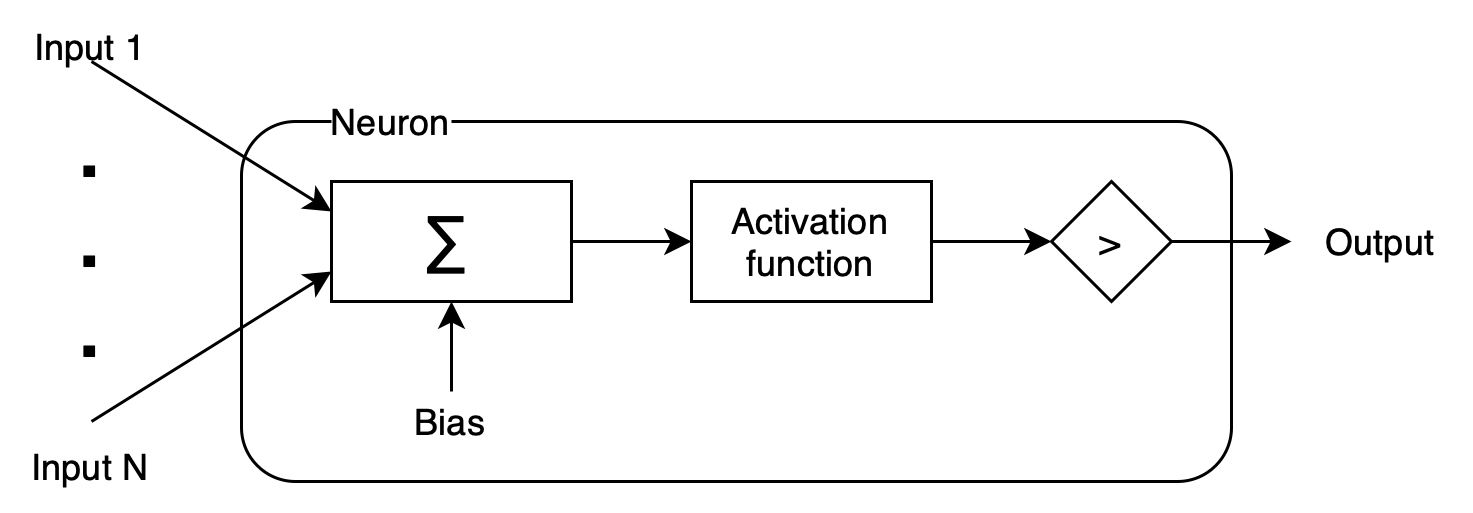
\includegraphics{thesis/images/neuron.png}
    \caption{Representation of a neuron in a neural network.}
    \label{fig:neuron}
\end{figure}

An artificial neural network is a set of neurons organized into layers.  Figure~\ref{fig:neural_network_example} represents a deep neural network, deep because there are one or more hidden layers. Different kinds of layers exist. The one shown in figure~\ref{fig:neural_network_example}, other than input and output, is a dense layer. In this kind of layer, every output of the previous layer is received as input by each neuron of the layer considered for the reasoning. Regarding the output layer, each neuron returns a probability that the input belongs to a class. When there is only one output neuron the probability is $p$ to belong to the class and $1-p$ to not belong to the class. When there is more than one neuron, each of them returns the probability of belonging to a class, and the highest one is taken as the prediction. A prediction, to be considered correct, must overcome a threshold value. In general, more are the hidden layer, more the network will be accurate but, more time will take to learn. 

\begin{figure}[H]
    \centering
    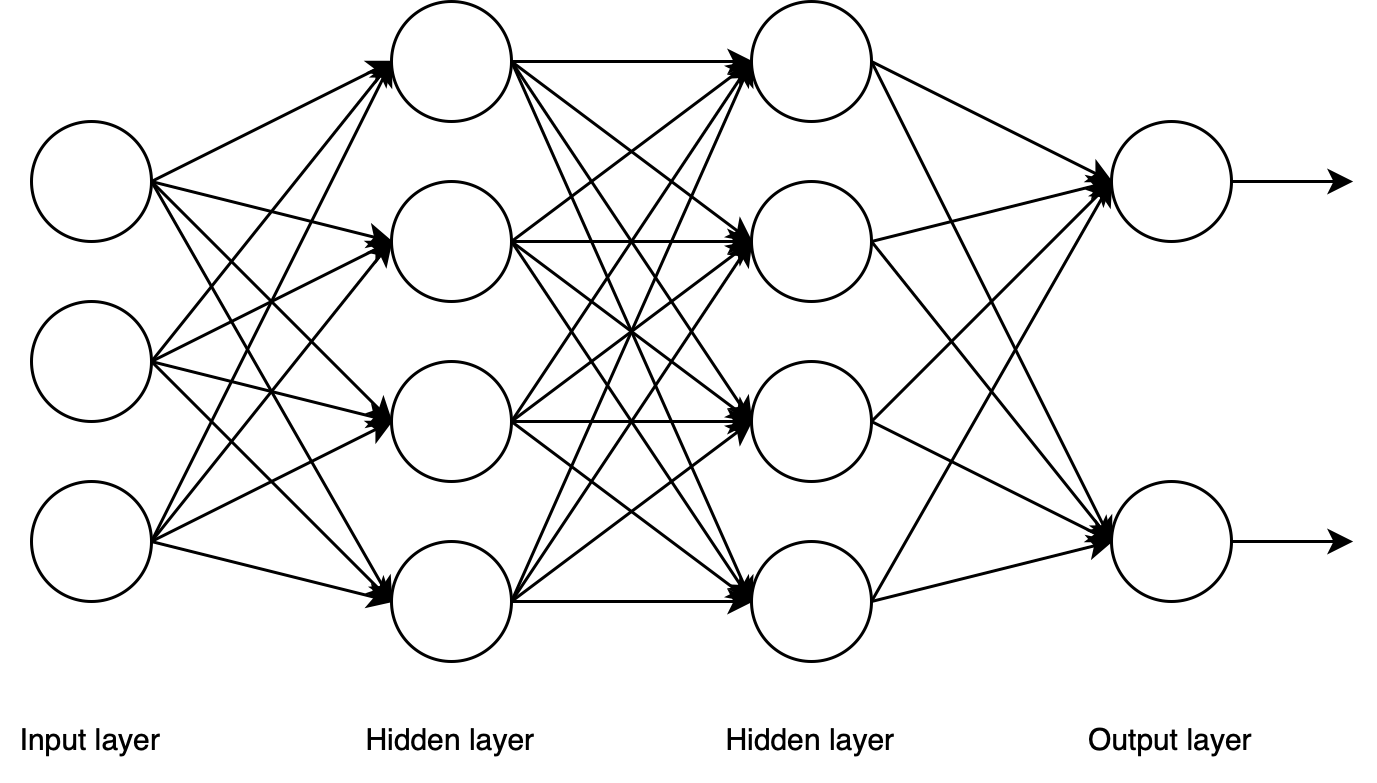
\includegraphics{thesis/images/neuralNetworkExample.png}
    \caption{An example of a deep neural network}
    \label{fig:neural_network_example}
\end{figure}

\subsubsection{Dataset}
When \acrshort{ML} is involved, one of the challenges is the need for large datasets on which the network can train. When image recognition is the task to be fulfilled, the datasets are composed of a lot of images, and each one must be labeled to know what it represents and where, inside the image, the position of the object to be detected is. This kind of training is known as supervised learning, which is different from unsupervised learning, in which the dataset has no labels and usually the task is to categorize the elements into macro-categories. Regarding the dataset dimension, it is worth to stress that the bigger the dataset, the slower the training task. It is important to find the right dimension that allows you to have an acceptable accuracy level. 

\subsubsection{Training}
The goal of training a neural network is to find the best weights for each neuron’s inputs. The technique for a multi-layer neural network is stochastic gradient descent with back propagation and data is essential to training a neural network. To correctly train and evaluate a neural network, three datasets are requested. Usually, one dataset is randomly divided into three non-overlapping partitions. The first and biggest part of the dataset is used to train the network. In more detail, it is used to adjust the weights of inputs. Then, another part of the dataset is picked as validation during the training process, and the last part is taken to evaluate the trained model at the end.

\subsubsection{Evaluation}
To evaluate an ML model, it is necessary to collect some data during the training process. The metrics to keep track of are: 
\begin{itemize}
    \item \textbf{loss function}: the network's goal is to minimize the loss function. Generally, it represents the prediction error with respect to the ground truth;
    \item \textbf{accuracy} is defined as the ratio of correct predictions to total predictions made.
        \begin{equation}
                Accuracy = \frac{Number\, of\, right\, predictions}{Number\, of\, predictions}
        \end{equation}
    \item \textbf{time}: the amount of time spent training the network. It depends on the dataset size and the complexity of the network. Specifically, a bigger dataset will require more time but will give better results, as well as a more complex network. 
\end{itemize}
The best neural network is the one that guarantees the best trade-off between these metrics. 

\subsubsection{State of the art}
With the help of neural networks, there are several ways to achieve good results in the hand gesture recognition task. The results presented in~\citeauthor{paper:survey_on_vision_based_hand_gesture_recognition}~\cite{paper:survey_on_vision_based_hand_gesture_recognition} shows that with a \acrfull{CNN}, it is possible to achieve an accuracy higher than  $90\%$. \acrshortpl{CNN} are classifier-based systems that can process input images as structured arrays of data and identify patterns between them. To date, there are two main types of object detection algorithms in the field of deep learning: 
\begin{itemize}
    \item \textbf{Classification-based algorithms}: firstly, they select a group of \acrfullpl{ROI} in the images where the chances that an object is present are high; secondly, they apply \acrshort{CNN} techniques to these selected regions to detect the presence of an object. A problem associated with these types of algorithms is that they need to execute a detector in each \acrshort{ROI}, and this makes the process of object detection very slow and highly expensive in terms of computation.
    \item \textbf{Regression-based algorithms}: these types of algorithms are faster than the above algorithms, in that there is no selection of the \acrshort{ROI} so that the bounding boxes and the labels are predicted for the whole image at once; they can identify and classify objects within the image at once. Beyond the higher speed, a key point is that the predictions are informed by the global context in the image, thus they generally lead to higher accuracies.
\end{itemize}
One of the most famous regression-based algorithms is \glsfirst{YOLO}, but it is not the only possible solution to perform this kind of task. Another technique that gives promising results is the combination of the MediaPipe hand tracker, which section~\ref{sec:mediapipe} describes, and a feed-forward neural network to recognize the gesture.\\ All these kinds of solutions suit well in the case of static hand gestures. As  \citeauthor{site:hand_gesture_base_repo} shows in his repository\cite{site:hand_gesture_base_repo}, working with a history of landmarks is possible. For this kind of task, a \glsfirst{LSTM} neural network is a good starting point. This kind of network tries to add the knowledge of past events to the computation. To do so, there are loops inside them that allow information to persist~\cite{site:understanding_lstm_networks}.

\section{Robot Operating System (ROS)}
\acrshort{ROS} was born as a framework to design robot software. Its initial presentation was in \citeyear{paper:ros} by \citeauthor{paper:ros}~\cite{paper:ros}. In particular it tries to solve the problem of communication but, it has also many other characteristics that make it a good framework for robot development.
\subsection{Communication}
A system based on \acrshort{ROS} has a \textit{peer-to-peer} topology. Each node of the network can communicate with any other node. The first version of \acrshort{ROS} implemented a custom communication layer but, from the second version onwards, it implements the \glsfirst{DDS} protocol.
\subsubsection{Data Distribution Service (DDS)}
\gls{ROS} uses \gls{DDS} as an end-to-end middleware to exchange messages: The adoption of the \gls{DDS} is one of the main differences between \gls{ROS} version 1 and \gls{ROS} version 2. The \gls{DDS} was chosen by the \gls{ROS} maintainer for its reliability and flexibility in mission-critical systems, such as:
\begin{itemize}
    \item battleships;
    \item extensive utility installations;
    \item monetary systems;
    \item spacecraft;
    \item flight control systems;
    \item train switchboard systems.
\end{itemize}
The implementation of \gls{DDS} is hidden from the user, who uses the methods described in section~\ref{sss:exchange_messages} with the \gls{ROS} API to exchange messages. A complete explanation for this change has been given by the developers and can be found on the article written by \citeauthor{site:ros_dds}~\cite{site:ros_dds}.

\subsection{Multi-lingual}
\gls{ROS} supports many programming languages. In particular C++ and Python are the most documented. Each supported language has its own implementation of the communication layer. In this way the developer can follow the best practice for each one but, it is possible to wrap the already written library into another language. ``The end result is a language-neutral message processing scheme where different languages can be mixed and matched as desired.''~\cite{paper:ros}

\subsection{Tools-based}
The developers of \gls{ROS} have decided to adopt a \textit{microkernel} design. In this way they produced different tools and, each of them perform a task:
\begin{itemize}
    \item navigate the source code tree;
    \item get and set configuration parameters;
    \item visualize the network topology;
    \item measure the band-with utilization;
    \item graphically plot message data;
    \item generate documentation;
    \item launch sequence of tasks
\end{itemize}
and many others.

\subsection{Thin}
\gls{ROS}' developers encourage the creation of small executables by leaving the complexity in the dependencies. This promotes writing code reusable also in other projects.

\subsection{Free and Open-Source}
\gls{ROS} is free and Open-Source, this has created a strong community around the framework. The community helps finding bugs and developing new algorithms accessible to everyone.

\subsection{Nomenclature}
The key points to understand when using \acrshort{ROS} are related to the ``ROS 2 Graph'', and they are:
\begin{itemize}
    \item \textbf{Node}: a system component in charge of a specific task. It is an executable, in my case, a Python executable, but it could also be a C++ executable, and it can communicate with other nodes, exchanging messages. A robotic system is composed of multiple nodes; 
    \item \textbf{Message}: the method by which nodes exchange data. Each message has its own ``type'', and this brings advantages in building an interchangeable system because it is possible to change the components of the system with others that can understand the same messages. Messages, in this case, can be seen as interfaces for programming languages. There are three ways for nodes to exchange messages: 
        \begin{itemize}
            \item \textbf{Topic};
            \item \textbf{Service};
            \item \textbf{Action}.
        \end{itemize}
\end{itemize}

\subsubsection{Exchange messages}\label{sss:exchange_messages}
\paragraph{Topic}\label{p:exchange_message_with_topics}
It is an implementation of the publisher/subscriber pattern. A node can publish messages with a topic, and every other node that is listening to that topic will read that message. This is an asynchronous way of exchanging messages because the sender will not know if the message has been read. For example, this is the best way to broadcast a message without saturating the network. 
\begin{figure}[H]
    \centering
    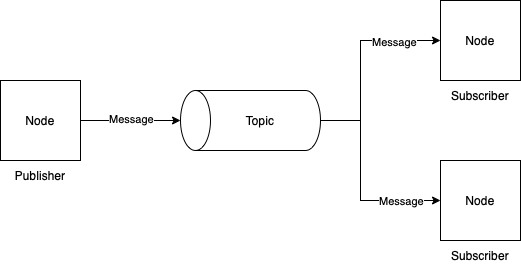
\includegraphics[width=0.7\columnwidth]{thesis/images/topicExample.png}
    \caption{Example of message exchange between three nodes using a topic.}
    \label{fig:exampleTopicExchangeMessage}
\end{figure}

\paragraph{Service}
It is based on a call-response model. In this case, a node requests some data from another node through a request message. The latter replies with a response message. This is a synchronous way of exchanging messages. The node that needs the data waits for the response. There can be many nodes that use the same service to request some data from another node. This is a bit like what happens in a client-server architecture, but it should not be used for long-running processes. 
\begin{figure}[H]
    \centering
    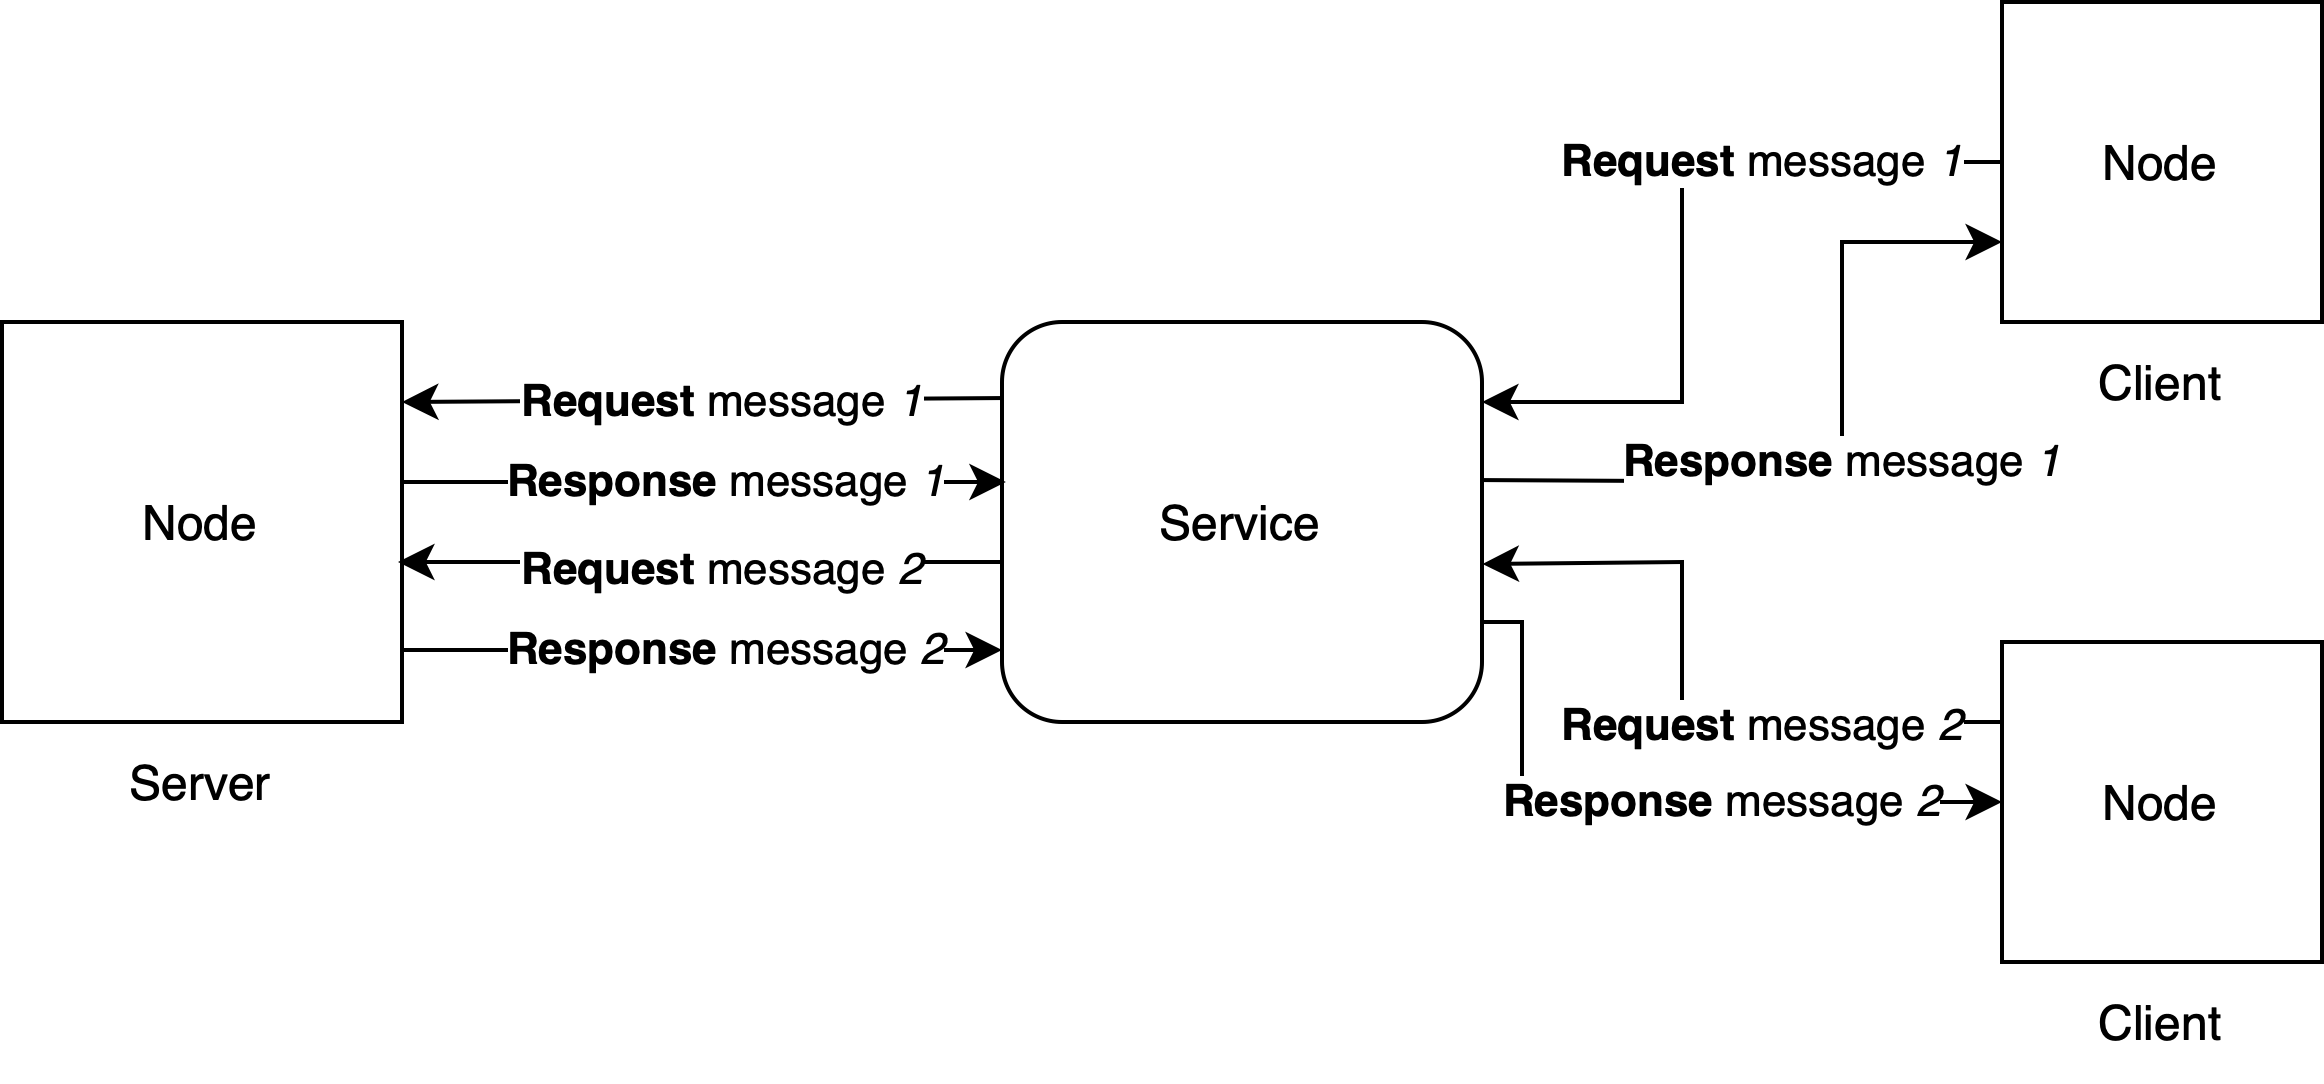
\includegraphics[width=0.8\columnwidth]{thesis/images/serviceExample.png}
    \caption{Example of messages exchange between three nodes using a service.}
    \label{fig:exampleServiceExchangeMessage}
\end{figure}

\paragraph{Action}\label{p:exchange_message_with_actions}
It uses both topics and services. The functionality is similar to service with the addition of a constant stream of updates from the ``server'' through a topic to which the ``client'' subscribes. The sequence of actions is the following: 
    \begin{enumerate}
        \item A node (i.e.\ the client) sends a message (the request for a goal) through a service to another node  (i.e.\ the server). The latter replies with one message through the service. For example, it can reply with an acknowledgment or a message saying it has started working on a task; 
        \item The server keeps the client updated with the progress of the task through a topic; 
        \item The client sends a request through another service to the server. When the task is finished, the server will reply to the client. 
    \end{enumerate}
\begin{figure}[H]
    \centering
    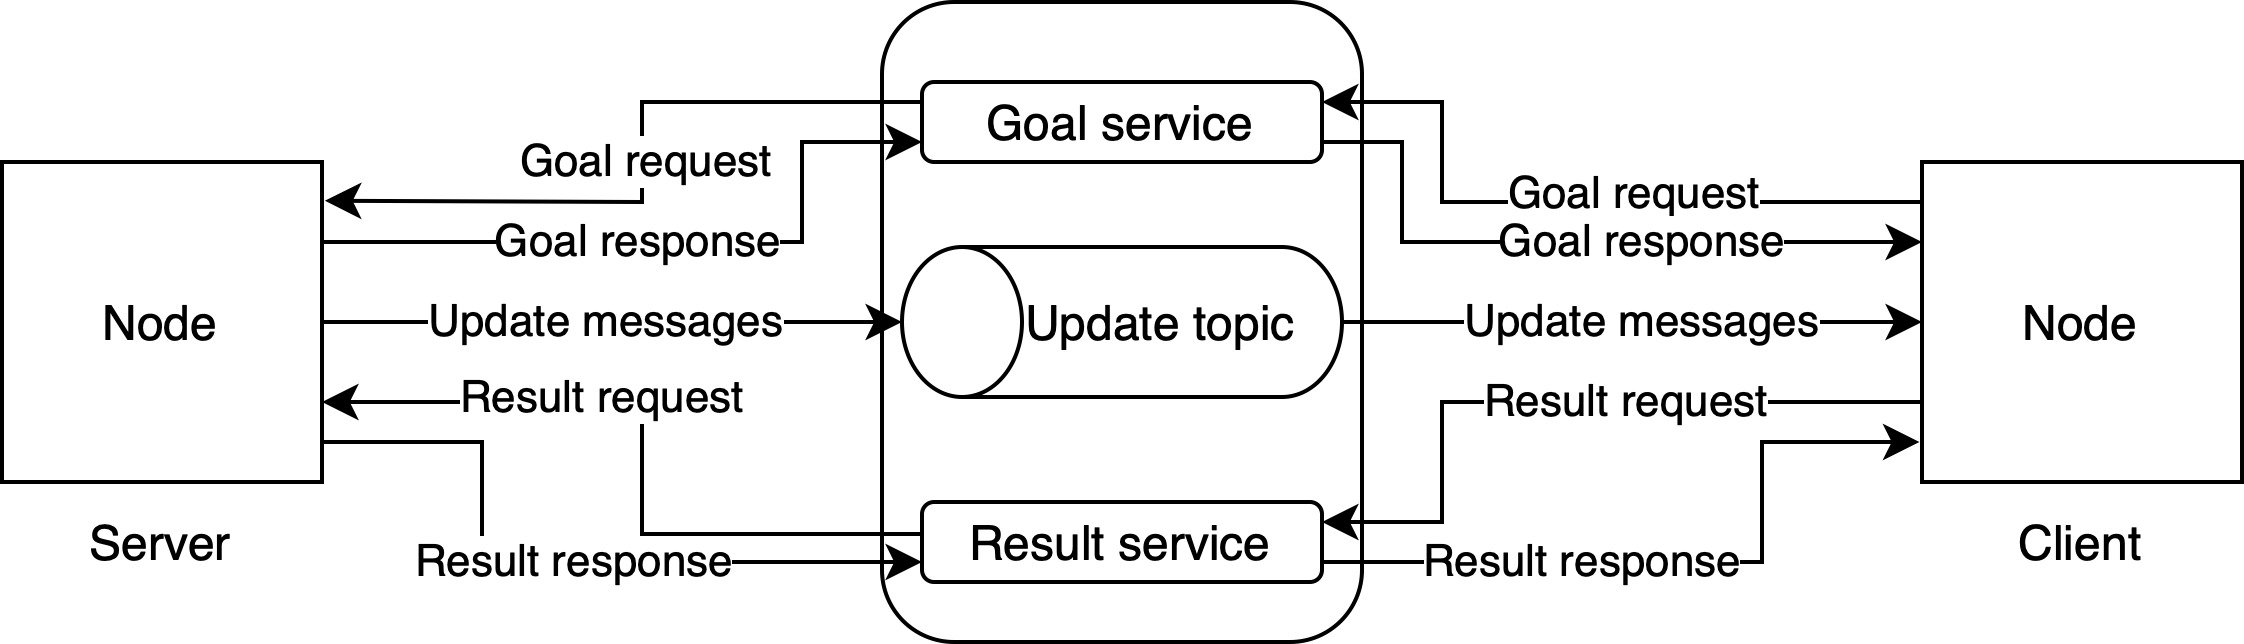
\includegraphics[width=1\columnwidth]{thesis/images/actionExample.png}
    \caption{Example of messages exchange between two nodes using an action.}
    \label{fig:exampleActionExchangeMessage}
\end{figure}

\end{document}
